\documentclass[12pt,a4paper]{article}

\usepackage[utf8]{inputenc}
\usepackage[T1]{fontenc}
\usepackage{lmodern}
\usepackage{microtype}
\usepackage{geometry}
\usepackage{xcolor}
\usepackage{booktabs}
\usepackage{tabularx}
\usepackage{longtable}
\usepackage{array}
\usepackage{enumitem}
\usepackage{fancyhdr}
\usepackage{titlesec}
\usepackage[most]{tcolorbox}
\usepackage{tikz}
\usepackage[hidelinks]{hyperref}

\usetikzlibrary{arrows.meta, positioning, shapes.geometric}

\geometry{margin=1in}
\setlength{\parindent}{0pt}
\setlength{\parskip}{0.75em}
\renewcommand{\arraystretch}{1.22}
\setlist[itemize]{leftmargin=1.4em}
\setlist[enumerate]{leftmargin=1.6em}

\definecolor{BUBlue}{HTML}{0089CB}
\definecolor{BUOrange}{HTML}{F97316}
\definecolor{BUSlate}{HTML}{0F172A}
\definecolor{BULight}{HTML}{F8FAFC}
\definecolor{BUGray}{HTML}{475569}

\hypersetup{
    colorlinks=true,
    linkcolor=BUBlue,
    urlcolor=BUBlue,
    citecolor=BUBlue,
    pdftitle={iBUConnect Project Documentation},
    pdfauthor={Exequiel Lustan}
}

\pagestyle{fancy}
\fancyhf{}
\lhead{\textbf{iBUConnect}}
\rhead{Project Documentation}
\cfoot{\thepage}
\renewcommand{\headrulewidth}{0.4pt}

\titleformat{\section}
  {\Large\bfseries\color{BUSlate}}
  {\thesection}{0.75em}{}
\titleformat{\subsection}
  {\large\bfseries\color{BUSlate}}
  {\thesubsection}{0.75em}{}
\titleformat{\subsubsection}
  {\normalsize\bfseries\color{BUSlate}}
  {\thesubsubsection}{0.75em}{}

\newcolumntype{Y}{>{\raggedright\arraybackslash}X}
\newcommand{\code}[1]{\texttt{#1}}

\tcbset{
    sharp corners,
    boxrule=0.6pt,
    colback=BULight,
    colframe=BUBlue!45!black,
    left=8pt,
    right=8pt,
    top=8pt,
    bottom=8pt
}

\begin{document}

\begin{titlepage}
    \centering
    \vspace*{2cm}
    {\Huge\bfseries\color{BUSlate} iBUConnect\par}
    \vspace{0.4cm}
    {\Large Project Documentation\par}
    \vspace{0.8cm}
    \rule{0.78\textwidth}{1pt}
    \vspace{1.2cm}

    \begin{tcolorbox}[width=0.78\textwidth,colback=white,colframe=BUBlue]
        \begin{tabularx}{\textwidth}{@{} l Y @{}}
            \textbf{Prepared by:} & Exequiel Lustan \\
            \textbf{Degree Program:} & Master of Information System \\
            \textbf{Institution:} & Bicol University \\
            \textbf{Academic Year:} & 2025--2026 \\
        \end{tabularx}
    \end{tcolorbox}

    \vfill
    {\large Bicol University\par}
    {\large Master of Information System Program\par}
\end{titlepage}

\tableofcontents
\newpage

\section{Executive Summary}

\textbf{iBUConnect} is a full-stack web application developed to modernize and centralize the handling of service requests across all administrative offices of Bicol University. The system replaces fragmented, paper-based, and email-driven workflows with a unified digital platform that provides real-time tracking, structured communication, document exchange, and data-driven accountability.

iBUConnect is built as a multi-surface platform: a \textbf{Public Information and Ticket Tracker} for unauthenticated users, a \textbf{Client Portal} for students and university personnel to submit and monitor requests, and an \textbf{Admin Panel} for office staff to process, assign, forward, and resolve those requests. The system is designed to scale across multiple offices while maintaining strict role-based access control and auditability.

\section{Problem Statement}

University administrative services traditionally rely on manual, in-person, or email-based processes for handling student and personnel requests. This approach presents several operational challenges:

\begin{itemize}
    \item \textbf{Lack of transparency} -- requesters have no visibility into the status or progress of their submitted requests.
    \item \textbf{Fragmented communication} -- correspondence is spread across email threads, physical forms, and verbal exchanges, making follow-ups difficult.
    \item \textbf{No accountability mechanism} -- there is no formal audit trail to attribute responsibility, track response times, or measure office performance.
    \item \textbf{Inefficient inter-office coordination} -- requests that require involvement from multiple offices have no structured handoff process, leading to duplicated effort or dropped requests.
    \item \textbf{Unstructured file management} -- document submissions are inconsistent, uncompressed, and difficult to retrieve.
\end{itemize}

\section{Project Objectives}

\begin{enumerate}
    \item Provide a centralized, role-aware digital platform for submitting, tracking, and resolving service requests.
    \item Implement a structured inter-office forwarding mechanism with transparent credit attribution for performance tracking.
    \item Deliver real-time bidirectional communication between requesters and office staff.
    \item Enforce a complete audit trail via a ticket history timeline for every state change.
    \item Automate file validation and optimize storage through a file management pipeline.
    \item Integrate university identity through Google OAuth to eliminate redundant account creation.
    \item Comply with Philippine data protection requirements by providing accessible legal documentation.
\end{enumerate}

\section{System Architecture}

iBUConnect follows a \textbf{monolithic full-stack architecture} built on the TALL stack (Tailwind CSS, Alpine.js, Laravel, Livewire), with a dedicated administration layer powered by Filament.

\begin{figure}[h]
\centering
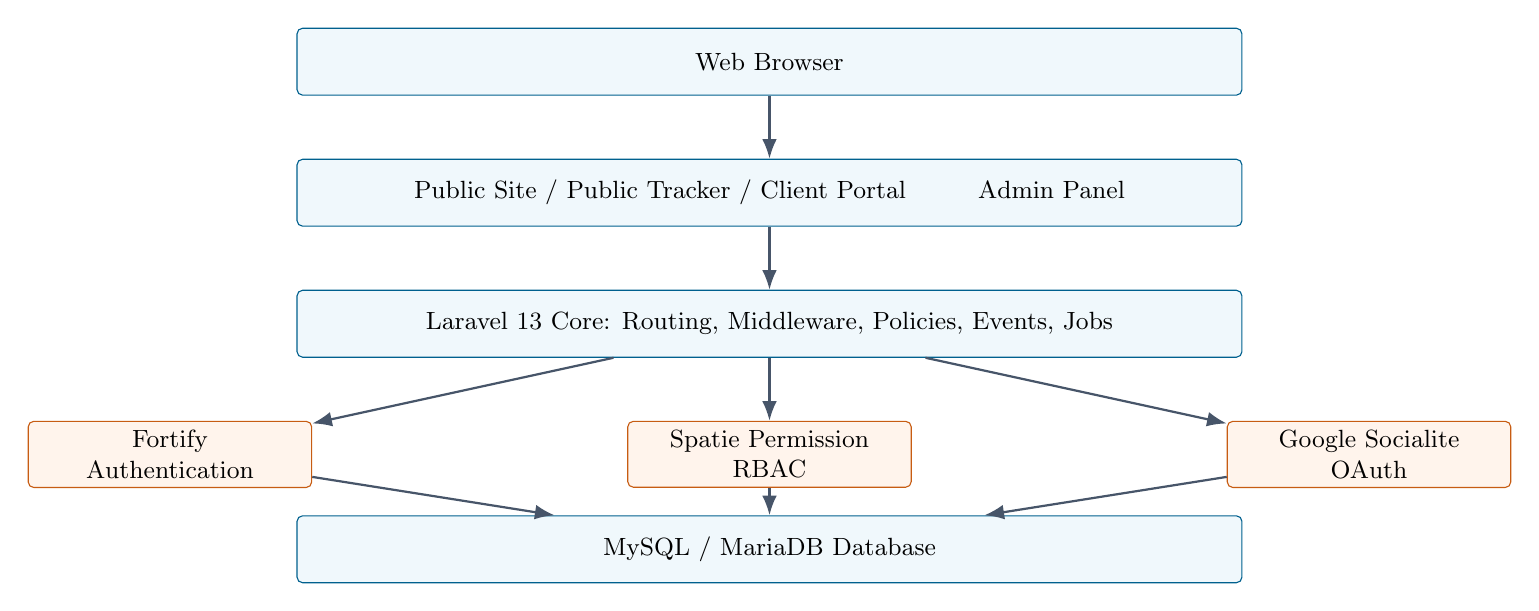
\begin{tikzpicture}[
    node distance=0.8cm,
    layer/.style={draw=BUBlue!70!black, fill=BUBlue!6, rounded corners=2pt, minimum width=12cm, minimum height=0.85cm, align=center, font=\small},
    sublayer/.style={draw=BUOrange!80!black, fill=BUOrange!8, rounded corners=2pt, minimum width=3.6cm, minimum height=0.8cm, align=center, font=\small},
    arrow/.style={-{Latex[length=2.5mm]}, thick, color=BUGray}
]
    \node[layer] (browser) {Web Browser};
    \node[layer, below=of browser] (surfaces) {Public Site / Public Tracker / Client Portal \hspace{0.7cm} Admin Panel};
    \node[layer, below=of surfaces] (laravel) {Laravel 13 Core: Routing, Middleware, Policies, Events, Jobs};
    \node[sublayer, below left=0.8cm and -0.2cm of laravel] (fortify) {Fortify\\Authentication};
    \node[sublayer, below=0.8cm of laravel] (spatie) {Spatie Permission\\RBAC};
    \node[sublayer, below right=0.8cm and -0.2cm of laravel] (socialite) {Google Socialite\\OAuth};
    \node[layer, below=2cm of laravel] (database) {MySQL / MariaDB Database};

    \draw[arrow] (browser) -- (surfaces);
    \draw[arrow] (surfaces) -- (laravel);
    \draw[arrow] (laravel) -- (fortify);
    \draw[arrow] (laravel) -- (spatie);
    \draw[arrow] (laravel) -- (socialite);
    \draw[arrow] (fortify) -- (database);
    \draw[arrow] (spatie) -- (database);
    \draw[arrow] (socialite) -- (database);
\end{tikzpicture}
\caption{High-level iBUConnect architecture}
\end{figure}

\subsection*{Request Flow}
\begin{enumerate}
    \item A user authenticates via Google OAuth or standard credentials.
    \item First-time users are guided through a structured onboarding flow before portal access is granted.
    \item Requests are submitted through a multi-step wizard and stored with a generated ticket identifier.
    \item Office staff manage requests through the Filament admin panel, with all state changes recorded to a history log.
    \item Requesters may also use the public \code{/track} page to verify a ticket by number and last name, view the public thread, reply as a guest, and upload requested documents.
    \item Real-time updates are delivered via Livewire's reactive component model, with \code{wire:poll} fallback for shared hosting.
\end{enumerate}

\section{Technology Stack}

\begin{table}[h]
\centering
\begin{tabularx}{\textwidth}{@{} l Y l @{}}
\toprule
\textbf{Layer} & \textbf{Technology} & \textbf{Version} \\
\midrule
Language & PHP & 8.4 \\
Framework & Laravel & 13 \\
Admin Panel & Filament & 5 \\
Frontend Reactivity & Livewire & 4 \\
UI Components & Flux UI (Livewire) & 2 \\
CSS Framework & Tailwind CSS & 4 \\
Authentication & Laravel Fortify & 1 \\
OAuth & Laravel Socialite & 5 \\
Authorization & Spatie Laravel Permission & 7 \\
Testing & Pest PHP & 4 \\
Code Quality & Laravel Pint & 1 \\
Development Tools & Laravel Sail, Pail & 1 \\
\bottomrule
\end{tabularx}
\end{table}

\section{Database Design}

The database is normalized around the ticket as the central entity. Key tables and their roles are described below.

\subsection{Core Tables}

\begin{longtable}{@{} p{0.28\textwidth} p{0.66\textwidth} @{}}
\toprule
\textbf{Table} & \textbf{Purpose} \\
\midrule
\endhead
\code{users} & University personnel and students; extended with Google OAuth and onboarding columns. \\
\code{offices} & University administrative units, each with configurable service offerings. \\
\code{service\_categories} & Logical groupings of services per office, such as Academic Records or Financial Aid. \\
\code{service\_types} & Individual requestable services with descriptions and document requirements. \\
\code{service\_type\_fields} & Dynamic form field definitions per service type, such as text, select, file, and checkbox inputs. \\
\code{tickets} & Central request record; stores status, priority, subject, custom field data, and timestamps. \\
\code{ticket\_histories} & Immutable audit log of every ticket state transition, assignment, and forwarding event. \\
\code{ticket\_messages} & Conversation thread per ticket, supporting public replies, guest replies, internal staff notes, and staff attachment requests. \\
\code{ticket\_attachments} & File uploads linked to a ticket or message, tracking disk location, MIME type, size, and nullable uploader for public tracker uploads. \\
\code{forwarding\_logs} & Records inter-office transfers including credit attribution and forwarding notes. \\
\code{canned\_responses} & Reusable message templates maintained by administrators for common replies. \\
\bottomrule
\end{longtable}

\subsection{Roles and Permissions}

Authorization is managed through Spatie Laravel Permission using the following roles:

\begin{table}[h]
\centering
\begin{tabularx}{\textwidth}{@{} l Y @{}}
\toprule
\textbf{Role} & \textbf{Scope} \\
\midrule
\code{super\_admin} & Full system access across all offices. \\
\code{office\_admin} & Administrative access scoped to their assigned office. \\
\code{staff} & Operational access to tickets within their office. \\
\code{client} & Portal access; can submit and track their own requests. \\
\bottomrule
\end{tabularx}
\end{table}

\section{System Modules}

\subsection{Public Information Module}

Accessible without authentication, this module presents a directory of university offices and their available services. Users may browse by office, view service descriptions and required documents, navigate directly to the request submission form for a specific service, track an existing ticket through \code{/track}, or review the system-wide workflow through the Project Overview page.

\textbf{Components:} \code{OfficeList}, \code{OfficeDetail}, \code{TicketTracker} (Livewire), public layout with legal pages, and \code{pages.project-overview}.

\subsubsection{Project Overview Page}

The \code{/project-overview} page provides a Cloudflare-inspired visual systems map for academic presentation and stakeholder review. It separates the system into tabbed workflow diagrams for submission, public tracking, staff work, forwarding, messaging, and reporting so each major function can be understood without overlapping arrows or mixed responsibilities.

The page is intentionally separate from the operational portal so evaluators can understand the complete system without needing a staff or student account. It includes:

\begin{itemize}
    \item Tabbed flowcharts for each major system function.
    \item Aligned left-to-right process steps that match the actual operational order.
    \item Data-written and visibility summaries for each workflow.
    \item A feature matrix covering the major modules.
    \item A data-path section showing how \code{tickets}, \code{ticket\_histories}, \code{ticket\_messages}, \code{ticket\_attachments}, and \code{forwarding\_logs} relate to each request.
\end{itemize}

\subsubsection{Public Ticket Tracker}

The public tracker allows requesters to access ticket status and conversation history without signing in. A requester enters the ticket number and their last name; successful verification stores the ticket ID in the session and shows only non-internal ticket details. From the tracker, requesters can:

\begin{itemize}
    \item View the ticket subject, office, service type, status, and public message thread.
    \item Reply to staff through guest messages stored with \code{sender\_id = null} and \code{guest\_name} set to the requester name.
    \item Upload documents only when a staff message has \code{requests\_attachment = true}.
    \item Clear the tracker session and search for another ticket.
\end{itemize}

The lookup flow uses Laravel's \code{RateLimiter} to reduce brute-force attempts and returns a generic error when either the ticket number or last name does not match.

\subsection{Authentication Module}

Supports dual authentication paths: Google OAuth, primarily using university accounts, and standard email/password with two-factor authentication. First-time users entering through Google OAuth are routed through a mandatory onboarding flow before gaining portal access.

\textbf{Components:} \code{GoogleAuthController}, \code{GoogleLogin} (Filament), Fortify configuration, and \code{EnsureOnboardingComplete} middleware.

\subsection{Client Portal Module}

The student and personnel-facing interface for submitting and monitoring service requests.

\textbf{Sub-modules:}
\begin{itemize}
    \item \textbf{Onboarding} -- Collects required profile information from new users before portal access.
    \item \textbf{Ticket Submission} -- A four-step wizard: Office, Category, Service Type, Form Fields, and Review, with dynamic field rendering per service type.
    \item \textbf{Ticket List} -- Paginated list of the authenticated user's tickets with status indicators.
    \item \textbf{Ticket Detail} -- Displays the full request, a vertical status timeline, and a public message thread with office staff.
\end{itemize}

\textbf{Components:} \code{CreateTicket}, \code{TicketList}, \code{TicketDetail}, \code{Onboarding}, and \code{OnboardingNotice}.

\subsection{Admin Panel Module}

The staff-facing management interface is built on Filament v5.

\subsubsection*{Filament Resources}
\begin{table}[h]
\centering
\begin{tabularx}{\textwidth}{@{} l Y @{}}
\toprule
\textbf{Resource} & \textbf{Manages} \\
\midrule
\code{TicketResource} & Ticket list, detail view, messaging, and status management. \\
\code{OfficeResource} & Office records and staff assignments. \\
\code{ServiceCategoryResource} & Service category configuration. \\
\code{ServiceTypeResource} & Service type definitions and dynamic form fields. \\
\code{UserResource} & User account management and role assignment. \\
\code{CannedResponseResource} & Reusable response templates. \\
\bottomrule
\end{tabularx}
\end{table}

\subsubsection*{Filament Actions}
\begin{table}[h]
\centering
\begin{tabularx}{\textwidth}{@{} l Y @{}}
\toprule
\textbf{Action} & \textbf{Function} \\
\midrule
\code{AssignTicketAction} & Assigns a ticket to a specific staff member with notifications. \\
\code{ForwardTicketAction} & Transfers a ticket to another office with credit attribution selection. \\
\bottomrule
\end{tabularx}
\end{table}

\textbf{Widgets:} \code{TicketStatsOverview}, a dashboard summary of pending, in-progress, and resolved ticket counts.

\subsection{Messaging Module}

A shared communication layer accessible from both the portal and the admin panel.

\begin{itemize}
    \item \textbf{Public Thread} -- Visible to both requester and staff.
    \item \textbf{Public Tracker Replies} -- Guest replies from \code{/track} are attributed with the requester's name and shown to staff with a ``Via public tracker'' badge.
    \item \textbf{Internal Notes} -- Staff-only annotations hidden from the requester.
    \item \textbf{Canned Responses} -- Staff may select pre-written templates to populate the message field.
    \item \textbf{Attachment Requests} -- Staff can flag a public reply as requesting an attachment, which exposes an upload form on the public tracker for that specific message.
    \item \textbf{Seen Indicators} -- Messages are marked with a timestamp when the recipient opens the ticket.
\end{itemize}

\subsection{Legal and Compliance Module}

Static pages fulfill institutional and regulatory transparency requirements under the Philippine Data Privacy Act.

\begin{table}[h]
\centering
\begin{tabularx}{\textwidth}{@{} l Y @{}}
\toprule
\textbf{Page} & \textbf{Content} \\
\midrule
Privacy Policy & Data collection, processing, and retention practices. \\
Terms of Service & Acceptable use and user obligations. \\
Data Protection Policy & Rights of data subjects and system safeguards. \\
Transparency Report & Institutional accountability statement. \\
Cookies Policy & Cookie usage disclosure. \\
\bottomrule
\end{tabularx}
\end{table}

\section{Key Features and Uniqueness}

\subsection{Dynamic, Service-Aware Request Forms}

Unlike static contact forms or generic ticketing systems, iBUConnect generates a tailored form for each service type. Administrators define custom fields such as text, number, dropdown, checkbox, and file upload per service without writing code. This allows the system to capture precisely the information each office requires for a given request.

\subsection{Structured Inter-Office Forwarding with Credit Attribution}

A distinguishing feature of iBUConnect is its formal inter-office forwarding mechanism. When a ticket must be handled by a different office, staff may forward it through a structured action that requires selecting a \textbf{credit type}:

\begin{itemize}
    \item \textbf{Accept Credit} -- Both the originating and receiving offices receive performance metric credit for the resolution.
    \item \textbf{Reference Only} -- Credit remains with the originating office; the receiving office acts in an advisory capacity.
\end{itemize}

Every forwarding action is recorded in a dedicated \code{forwarding\_logs} table with full metadata, enabling objective institutional performance measurement that is not possible in informal routing workflows.

\subsection{Immutable Ticket History Timeline}

Every meaningful event in a ticket's lifecycle, including creation, assignment, status change, forwarding, note addition, resolution, and closure, is recorded as an immutable row in the \code{ticket\_history} table. This timeline is rendered as a visual, vertical progress tracker in the client portal, giving requesters full transparency into what happened to their request and when.

\subsection{Auto-Generated Structured Ticket Identifiers}

Each ticket receives a human-readable identifier generated from the office acronym, a type code, and a sequential number, such as \code{OADA-T-26-0001}. This makes verbal and written reference to specific requests unambiguous across offices and communication channels.

\subsection{Public Ticket Tracking Without Account Friction}

iBUConnect includes a public \code{/track} page for requesters who need to follow up without logging in. The tracker uses ticket number plus requester last-name verification, stores the verified ticket in the PHP session, and reveals only public ticket details. This keeps follow-up lightweight while preserving privacy controls for internal staff notes.

\subsection{Staff-Requested Guest Attachments}

Office staff can request an attachment directly from a public reply. When that flag is set, the public tracker displays an upload control scoped to the requesting message. Uploaded files are linked back to the ticket and message with a nullable uploader, making it clear that the file came from the public tracker rather than an authenticated account.

\subsection{Onboarding Gate with Middleware Enforcement}

New users authenticated through Google are not immediately granted portal access. A dedicated onboarding flow collects institutional profile information before the \code{EnsureOnboardingComplete} middleware grants access to protected routes. This ensures data completeness for all active accounts.

\subsection{Role-Scoped Staff Access}

Staff accounts are restricted by office membership enforced at the policy and query level. A staff member cannot view, respond to, or act on tickets belonging to another office. This access control model mirrors real-world institutional boundaries and prevents information leakage between departments.

\subsection{Internal Notes Invisible to Requesters}

The messaging module supports an internal note toggle that renders staff communications invisible to the requester. This allows teams to coordinate, escalate, or annotate tickets without exposing deliberative content to end users, a common requirement in professional service desk operations.

\section{Security and Compliance}

\begin{longtable}{@{} p{0.32\textwidth} p{0.62\textwidth} @{}}
\toprule
\textbf{Concern} & \textbf{Implementation} \\
\midrule
\endhead
Authentication & Google OAuth plus Fortify support for password and two-factor authentication. \\
Authorization & Spatie Permission RBAC and model policies per resource. \\
SQL Injection & Eloquent ORM with parameterized queries throughout. \\
Mass Assignment & PHP 8.4 \code{\#[Fillable]} attribute on all models. \\
Soft Deletes & Tickets use \code{SoftDeletes}; historical data is preserved. \\
Input Validation & Server-side validation on all Livewire and Filament actions. \\
File Uploads & MIME type and size validation on all attachment inputs. \\
Session Security & Laravel session management and CSRF protection on all forms. \\
Public Tracker Protection & Ticket lookup requires ticket number plus requester last name, uses generic mismatch errors, and is rate-limited. \\
Data Privacy & Compliant legal pages per the Philippine Data Privacy Act. \\
Onboarding Gate & Middleware blocks portal access until profile is complete. \\
\bottomrule
\end{longtable}

\section{Benefits and Impact}

\subsection{For Students and University Personnel}
\begin{itemize}
    \item Eliminates the need for in-person follow-ups or repeated email inquiries.
    \item Provides a single interface to track all submitted requests and their current status.
    \item Allows public ticket follow-up by ticket number and last name when a full portal sign-in is unnecessary.
    \item Delivers a chronological timeline of every action taken on a request.
    \item Enables direct, documented communication with the responsible office.
    \item Supports staff-requested document uploads from the public tracker.
\end{itemize}

\subsection{For Office Staff}
\begin{itemize}
    \item Replaces unstructured email inboxes with a prioritized, filterable ticket queue.
    \item Reduces repetitive typing through canned response templates.
    \item Enables clean handoffs to other offices through the forwarding mechanism.
    \item Provides internal annotation capability without exposing deliberations to requesters.
    \item Allows staff to request specific attachments from requesters and see public tracker replies clearly attributed.
\end{itemize}

\subsection{For University Administration}
\begin{itemize}
    \item Centralizes all service request data into a single queryable system.
    \item Enables office performance measurement through credit attribution on inter-office forwarding.
    \item Produces an auditable history of every action taken across all offices.
    \item Reduces paper consumption and manual filing overhead.
    \item Supports evidence-based decisions on staffing and service load distribution.
\end{itemize}

\section{Conclusion}

iBUConnect addresses a concrete institutional need: the absence of a structured, transparent, and accountable digital workflow for university service requests. By combining a public tracker, client-facing portal, and staff-facing administration panel under a single, integrated codebase, iBUConnect provides a coherent experience for all stakeholders while maintaining strict separation of concerns at the data and authorization layers.

The system's distinguishing contributions -- structured inter-office forwarding with credit attribution, an immutable ticket history timeline, service-aware dynamic forms, public ticket tracking, staff-requested attachments, and role-scoped access control -- address limitations not typically found in generic help desk solutions. These features reflect the specific operational realities of a multi-office academic institution and position iBUConnect as a purpose-built solution rather than a repurposed commercial tool.

The architecture is designed for deployability on Hostinger shared hosting or VPS environments, with Livewire's polling mechanism as a fallback for real-time updates, ensuring practical viability within the university's existing infrastructure constraints.

\vfill
\begin{center}
    \textit{Document prepared for academic project presentation purposes.}\\
    \textit{Bicol University -- Master of Information System Program}
\end{center}

\end{document}
